\documentclass[a4paper]{article}
\usepackage{latexsym,amssymb,amsmath,amsbsy,amsopn,amstext,xcolor,multicol}
\usepackage{ctex,hyperref,graphicx,wrapfig,fancybox,listings,subfigure}
\usepackage{pgf,pgfarrows,pgfnodes,pgfautomata,pgfheaps,pgfshade}
\usepackage[top=1in, bottom=1in, left=1.25in, right=1.25in]{geometry}
\graphicspath{{pic/}}
\lstset{numbers=left,
keywordstyle=\color{blue!70}, commentstyle=\color{red!50!green!50!blue!50},
frame=shadowbox,
rulesepcolor=\color{red!20!green!20!blue!20},
breaklines=true,
extendedchars=true
}
\renewcommand{\figurename}{图}
\title{\bf Image Fusion}
\date{2018.6}
\author{计64~~翁家翌~2016011446}
\begin{document}
\kaishu
\ttfamily
\maketitle
\tableofcontents
\newpage

\section{运行说明}
首先安装依赖的第三方库:
\begin{lstlisting}[language=bash]
sudo apt install cmake libcgal-dev libcgal-qt5-dev
sudo pip2 install opencv-python
\end{lstlisting}

然后编译C++文件:
\begin{lstlisting}[language=bash]
cmake .
make
\end{lstlisting}
在当前目录下生成可执行文件 \underline{main}。

使用命令
\begin{lstlisting}[language=bash]
./main <args>
\end{lstlisting}
即可运行或查看帮助,如图\ref{fig:2-1}所示:
\begin{figure}[htp]
\centering
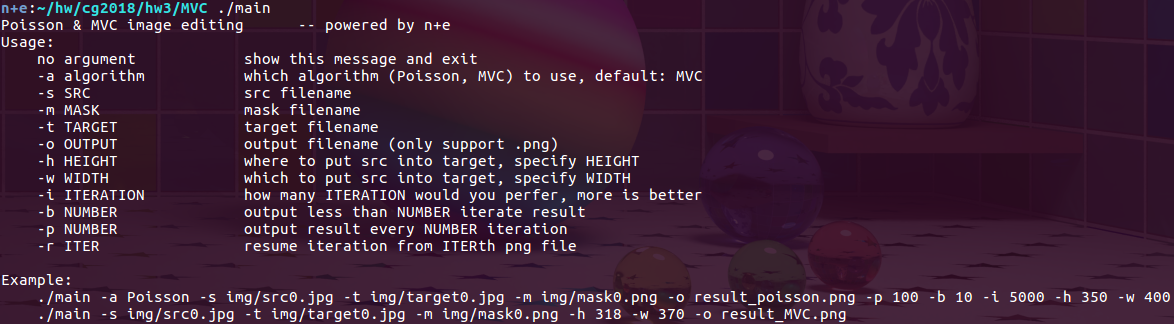
\includegraphics[width=1\linewidth]{2_1.png}
\caption{查看帮助}
\label{fig:2-1}
\end{figure}

\section{实现方式}

考虑到实现效率,我采用C++编写代码,其中图片的读入和输出采用github上的开源仓库"stb"\footnote{\url{https://github.com/nothings/stb}}实现,图片边缘的提取采用OpenCV\footnote{\url{https://opencv.org/}}。

\section{算法细节}
\subsection{MVC}
MVC\cite{MVC,MVC2}算法可分为如下步骤:
\begin{enumerate}
	\item 找出所有的边缘像素点的位置;
	\item 使用CGAL将这些点进行带约束的三角剖分;
	\item 对于三角剖分结果中的非边缘像素点,依据论文中给出的权重计算方式算出这个点所要垫高的权值;
	\item 对于每个三角面片,已经求出了三个顶点的垫高的权值,并且由于假设函数在该范围内平滑,因此直接用一个平面去拟合三角形内的所有像素点的权值大小即可。
\end{enumerate}

\subsection{Poisson}
此外我还实现了泊松图像融合算法\cite{PS,PS2}进行对比,其梯度计算方式为
$$
\nabla(x,y)=4I(x,y)-I(x-1,y)-I(x,y-1)-I(x+1,y)-I(x,y+1)
$$

将原图求完梯度之后,将该梯度匹配到目标图上的某一区域,本质上是一个解线性方程组的问题。形式化地,设有$N$个像素点需要匹配到目标图片中,则需要求解线性方程组
$$
A\vec{x}=\vec{b}
$$

其中$\vec{x}$代表融合后的图片中像素点的值,矩阵$A$的大小$\sim N\times N$,列向量$\vec{x}$和$\vec{b}$的大小$\sim N$,并且$A$的每一行至多只有5个非零元素,并且对角线上的元素均为4。

$A$是一个巨大的稀疏矩阵。考虑到矩阵求逆的复杂度为$O(N^3)$太高,并且某些情况下连$A$都无法直接以矩阵形式存储,因此无法直接从公式
$$
\vec{x}=A^{-1}\vec{b}
$$
求得$\vec{x}$。此处采用Jacobi Method迭代求解出$\vec{x}$的值,详见\cite{JB}。
\subsection{实验结果}
\subsubsection{Test1}
使用命令
\begin{lstlisting}[language=bash]
time ./main -s img/src3.jpg -t img/target1.jpg -m img/mask3.jpg -o result_MVC.png -h -135 -w -30 -a MVC
time ./main -s img/src3.jpg -t img/target1.jpg -m img/mask3.jpg -o result_Poisson.png -i 5000 -h 50 -w 100 -a Poisson
\end{lstlisting}

可得到如下结果
\begin{lstlisting}[language=bash]
Done with 262 vertices and 466 triangles.
real	0m0.243s
user	0m0.287s
sys	0m0.233s
------
iter 5001  err 0.001767 0.001913 0.003486
real	0m0.361s
user	0m0.345s
sys	0m0.016s
\end{lstlisting}

可以看到,MVC总共只用了262个三角顶点,耗时0.243s;Poisson由于使用迭代方法求解矩阵,迭代次数越多解的越精确,5000轮之后误差几乎为0,并且运行速度为0.36s,二者均十分快。合成效果如图\ref{fig:2-2}所示。由于该样本太容易合成,二者在效果上看不出有什么明显差别。
\begin{figure}[htp]
\centering
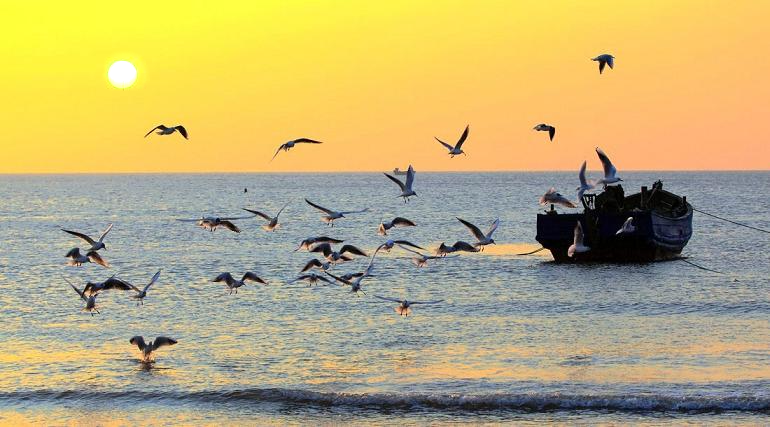
\includegraphics[width=0.8\linewidth]{2_2.png}
\caption{第一组数据合成效果}
\label{fig:2-2}
\end{figure}

\subsubsection{Test2}
使用命令
\begin{lstlisting}[language=bash]
time ./main -s img/src4.png -t img/target2.png -m img/mask4.png -o result_MVC.png -h 142 -w 132 -a MVC
time ./main -s img/src4.png -t img/target2.png -m img/mask4.png -o result_Poisson.png -i 10000 -h 150 -w 150 -a Poisson
\end{lstlisting}
可得到如下结果
\begin{lstlisting}[language=bash]
Done with 836 vertices and 1580 triangles.
real	0m0.233s
user	0m0.228s
sys	0m0.305s
------
iter 10001  err 82.519269 49.665685 58.341544
real	0m5.356s
user	0m5.351s
sys	0m0.004s
\end{lstlisting}

可以看到MVC总共只用了836个三角顶点,耗时0.228s;Poisson在10000轮之后总误差不到100,平均每个像素点误差不到0.01,并且运行速度为5s左右。合成效果如图\ref{fig:2-4}所示,对比可以发现MVC的边缘比Poisson更加平滑。

\begin{figure}[htp]
\centering
\subfigure[MVC]
{
\begin{minipage}[b]{0.45\columnwidth}
\centering
\resizebox{\columnwidth}{!}{
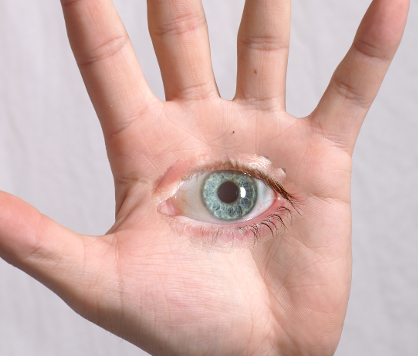
\includegraphics[width=1\columnwidth]{2_3.png} 
}
\label{fig:2-4:a}
\end{minipage}
}
\hfil
\subfigure[Poisson]
{
\begin{minipage}[b]{0.45\columnwidth}
\centering
\resizebox{\columnwidth}{!}{
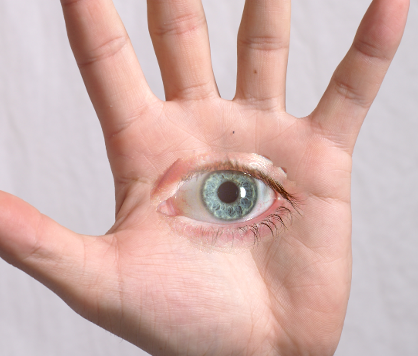
\includegraphics[width=1\columnwidth]{2_4.png}
}
\label{fig:2-4:b}
\end{minipage}
}
\caption{第二组数据合成效果}
\label{fig:2-4}
\end{figure}

\subsubsection{Test3}
使用命令
\begin{lstlisting}[language=bash]
time ./main -s img/src0.jpg -t img/target0.jpg -m img/mask0.png -h 318 -w 370 -o result_MVC.png
time ./main -a Poisson -s img/src0.jpg -t img/target0.jpg -m img/mask0.png -o result_poisson.png -i 10000 -h 350 -w 400
\end{lstlisting}
可得到如下结果
\begin{lstlisting}[language=bash]
Done with 1702 vertices and 3346 triangles.
real	0m0.420s
user	0m0.458s
sys	0m0.253s
------
iter 10001  err 2238.275301 1683.477450 1885.838338
real	0m43.901s
user	0m43.816s
sys	0m0.040s
\end{lstlisting}

这是MVC论文中的图,可以看到MVC总共只用了1702个三角顶点,耗时0.458s;Poisson在10000轮之后总误差大约2000,平均每个像素点误差不到0.03,但是运行速度达到了43s左右。合成效果如图\ref{fig:2-5}所示。从效果上看而言还是MVC更胜一筹。

\begin{figure}[htp]
\centering
\subfigure[MVC]
{
\begin{minipage}[b]{0.45\columnwidth}
\centering
\resizebox{\columnwidth}{!}{
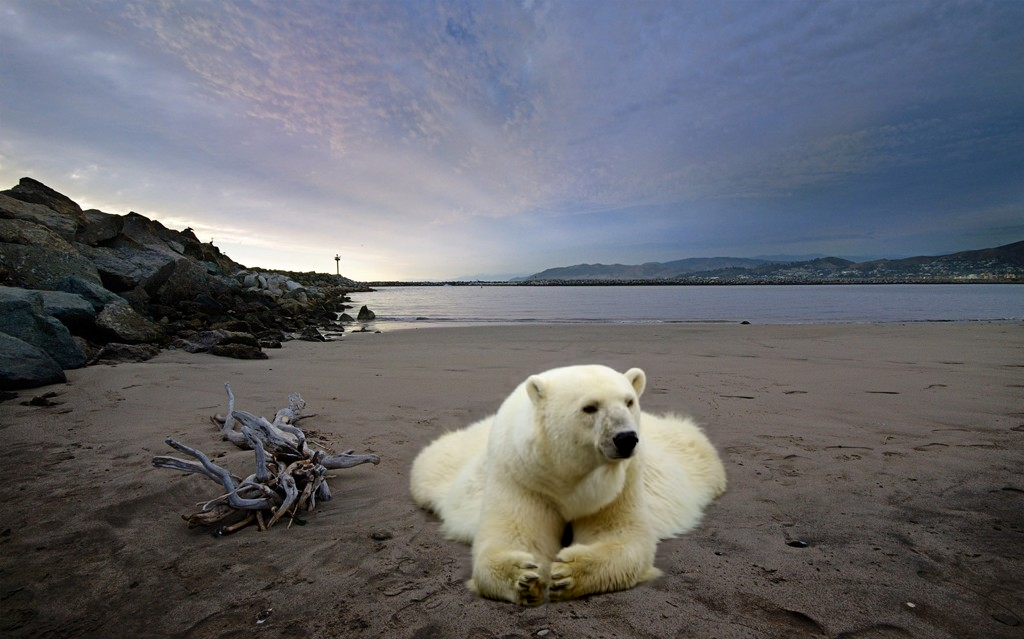
\includegraphics[width=1\columnwidth]{2_5.png} 
}
\label{fig:2-5:a}
\end{minipage}
}
\hfil
\subfigure[Poisson]
{
\begin{minipage}[b]{0.45\columnwidth}
\centering
\resizebox{\columnwidth}{!}{
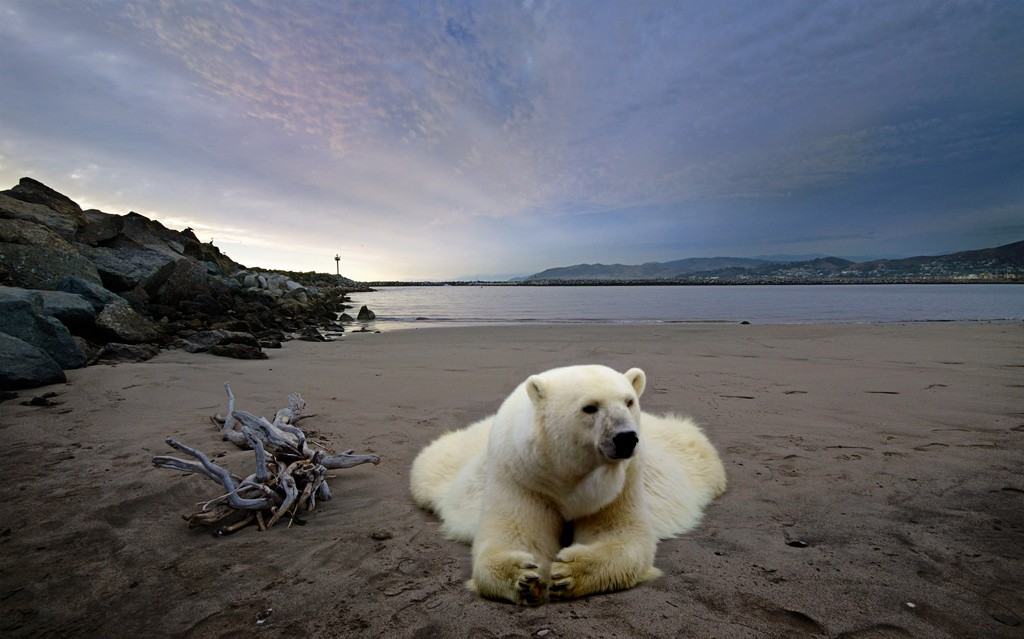
\includegraphics[width=1\columnwidth]{2_6.png}
}
\label{fig:2-5:b}
\end{minipage}
}
\caption{第三组数据合成效果}
\label{fig:2-5}
\end{figure}

\newpage 
\bibliography{report.bib}{}
\bibliographystyle{plain}
\end{document}
